\section{Pendahuluan}
\subsection{Latar Belakang}
Jaringan komputer merupakan tulang punggung dari sistem komunikasi modern, memungkinkan perangkat untuk saling bertukar informasi melalui berbagai media transmisi. Dalam perkembangan teknologi saat ini, pemahaman terhadap bagaimana data berpindah dalam jaringan menjadi sangat penting, terutama bagi mahasiswa Teknik Komputer. Praktikum Jaringan Komputer merupakan sarana pembelajaran praktis yang bertujuan untuk memberikan pengalaman langsung dalam mengamati dan menganalisis lalu lintas jaringan menggunakan berbagai tools.
\\ Modul 1 praktikum ini berfokus pada pengenalan dan penggunaan aplikasi Wireshark, sebuah network protocol analyzer yang sangat umum digunakan untuk menangkap dan menganalisis paket data yang melintasi jaringan. Melalui praktikum ini, mahasiswa diharapkan dapat memahami struktur dasar paket, mengenali berbagai protokol yang digunakan (seperti HTTP, DNS, ICMP, dan lainnya), serta menganalisis cara kerja komunikasi data secara langsung. Pemahaman ini menjadi bekal penting dalam mendalami aspek-aspek teknis jaringan komputer serta troubleshooting jaringan secara profesional.

\subsection{Dasar Teori}
\begin{enumerate}
    \item Crimping Kabel Jaringan
    \\Crimping adalah proses penyambungan konektor ke ujung kabel jaringan menggunakan alat crimping. Tujuan dari crimping adalah untuk menghasilkan koneksi fisik yang baik antara kabel dan konektor agar dapat digunakan untuk mentransmisikan data. Jenis kabel yang umum digunakan dalam jaringan komputer adalah kabel twisted pair (UTP/STP) dengan konektor RJ-45.
    \\Terdapat dua standar penyusunan kabel jaringan, yaitu:
    \begin{itemize}
        \item Straight-through: digunakan untuk menghubungkan perangkat yang berbeda, misalnya PC ke switch.
        \item Crossover: digunakan untuk menghubungkan perangkat yang sama, misalnya PC ke PC.
    \end{itemize}
    Proses crimping melibatkan langkah-langkah seperti pengupasan kabel, penyusunan warna kabel sesuai standar (TIA/EIA-568A atau TIA/EIA-568B), dan menekan konektor dengan alat crimping agar koneksi kuat dan stabil.
    \item Routing IPv4
    \\Routing adalah proses pengiriman paket data dari satu jaringan ke jaringan lain melalui perangkat yang disebut router. Proses ini sangat penting dalam jaringan berskala besar atau yang terdiri atas banyak subnet.
    \\IPv4 (Internet Protocol version 4) adalah protokol komunikasi yang digunakan untuk mengidentifikasi perangkat di jaringan menggunakan alamat 32-bit yang dibagi ke dalam empat oktet (misalnya, 192.168.1.1). Routing IPv4 mengatur bagaimana data dikirimkan dari satu alamat IP ke alamat IP lainnya.
    \\Terdapat dua jenis routing:
    \begin{itemize}
        \item Static Routing: rute ditentukan secara manual oleh administrator jaringan. Cocok untuk jaringan kecil dan tetap.
        \item Dynamic Routing: rute ditentukan secara otomatis menggunakan protokol seperti RIP, OSPF, atau EIGRP. Cocok untuk jaringan besar yang bersifat dinamis.
    \end{itemize}
    Routing pada IPv4 membutuhkan pengaturan alamat IP pada setiap antarmuka router dan konfigurasi tabel routing agar router mengetahui ke mana paket harus diteruskan.
\end{enumerate}



%===========================================================%
\section{Tugas Pendahuluan}
\begin{enumerate}
Sebuah perusahaan baru sedang membangun jaringan internal yang akan dibagi menjadi beberapa bagian berdasarkan departemen. Setiap departemen akan memiliki jaringan lokalnya sendiri dan akan saling terhubung melalui sebuah router utama. Berikut adalah informasi mengenai jumlah perangkat yang digunakan masing-masing departemen:

\begin{itemize}
    \item Departemen Produksi: 50 perangkat
    \item Departemen Administrasi: 20 perangkat
    \item Departemen Keuangan: 10 perangkat
    \item Departemen R&D: 100 perangkat
\end{itemize}

Administrator jaringan diminta untuk:
\begin{itemize}
    \item Membuat perencanaan alokasi IP address untuk masing-masing departemen.
    \item Menentukan prefix subnet (CIDR) yang paling sesuai untuk masing-masing kebutuhan, tanpa memboroskan IP.
    \item Memastikan tidak ada overlap antar subnet.
    \item Membuat skema routing agar masing-masing jaringan bisa saling berkomunikasi melalui router, jika diperlukan.
\end{itemize}


	\item Tentukan:
    \begin{itemize}
        \item Rentang IP address dan prefix (CIDR) yang sesuai untuk masing-masing departemen.
        \item Total subnet yang diperlukan dan IP network untuk masing-masing.
    \end{itemize}
    
    Jawaban:
    \\Menentukan prefix CIDR yang tepat berdasarkan jumlah perangkat:
    \begin{table}[h]
    \centering
    \label{tabel1}
    \begin{tabular}{|c|c|c|c|c|}
      \hline
      Departemen & Jumlah Perangkat & IP yang Dibutuhkaan & Prefix CIDR & Jumlah IP Tersedia \\
      \hline
      Produksi & 50 & 50 + beberapa cadangan & /26 & 64 IP \\
      Administrasi & 20 & 20 + beberapa cadangan & /27 & 32 IP \\
      Keuangan & 10 & 10 + beberapa cadangan & /28 & 16 IP \\
      R and D & 100 & 100 + beberapa cadangan & /25 & 128 IP \\
      \hline
    \end{tabular}
    \caption{Penentuan prefix CIDR berdasarkan jumlah perangkat tiap departemen dan kebutuhan cadangan IP}
    \end{table}
    
    Menggunakan alamat jaringan privat 192.168.0.0/24 dan membaginya:
    \begin{table}[H]
    \centering
    \begin{tabular}{|c|c|c|c|c|}
      \hline
      Departemen & Subnet & Range IP & Broadcast & Gateway \\
      \hline
      Produksi & 192.168.1.0/26 & 192.168.1.1 - 192.168.1.62 & 192.168.1.63 & 192.168.1.1 \\
      Administrasi & 192.168.1.64/27 & 192.168.1.65 - 192.168.1.94 & 192.168.1.95 & 192.168.1.65 \\
      Keuangan & 192.168.1.96/28 & 192.168.1.97 - 192.168.1.110 & 192.168.1.111 & 192.168.1.97 \\
      R and D & 192.168.1.112/25 & 192.168.1.113 - 192.168.1.254 & 192.168.1.255 & 192.168.1.113 \\
      \hline
    \end{tabular}
    \caption{Pembagian subnet untuk tiap departemen}
    \end{table}
    
    \item Gambarkan topologi sederhana yang menunjukkan bagaimana router akan menghubungkan semua subnet.
    \begin{figure}[htbp] 
        \centering  
        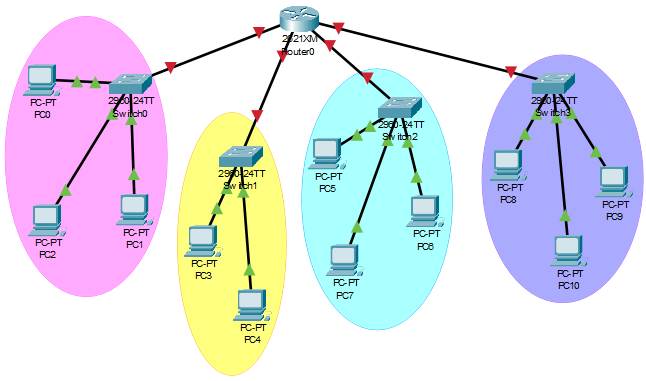
\includegraphics[width=1\textwidth]{Template Laporan Sementara/P1/img/cisco.png}  
        \caption{Topologi Jaringan} 
        \label{fig:nama_gambar} 
    \end{figure}
    
	\item Tuliskan tabel routing sederhana yang menunjukkan:
    \begin{itemize}
        \item Network destination
        \item Netmask/prefix
        \item Gateway (anggap antarmuka router)
        \item Interface tujuan
    \end{itemize}
    Jawaban :
    \\Berikut adalah tabel routing yang diperlukan pada router utama:
    \begin{table}[H]
    \centering
    \begin{tabular}{|c|c|c|c|}
      \hline
      Network Destination & Netmask/Prefix & Gateway & Interface \\
      \hline
      192.168.1.0 & 255.255.255.192 (/26) & - & eth0 \\
      192.168.1.64 & 255.255.255.224 (/27) & - & eth2 \\
      192.168.1.96 & 255.255.255.240 (/28) & - & eth1 \\
      192.168.1.112 & 255.255.255.128 (/25) & - & eth3 \\
      0.0.0.0 & 0.0.0.0 (/0) & ISP Gateway & WAN Interface \\
      \hline
    \end{tabular}
    \caption{Tabel routing pada router utama yang menunjukkan network destination, netmask/prefix, gateway, dan interface tujuan}
    \end{table}
    Pada setiap jaringan departemen, konfigurasi default gateway mengarah ke interface router utama:
    \begin{itemize}
        \item Departemen Produksi: Default gateway 192.168.1.1
        \item Departemen Administrasi: Default gateway 192.168.1.65
        \item Departemen Keuangan: Default gateway 192.168.1.97
        \item Departemen R&D: Default gateway 192.168.1.113
    \end{itemize}

    \item Berdasarkan topologi yang telah kamu buat, jenis routing apa yang paling cocok untuk perusahaan ini? Jelaskan alasanmu secara rinci. Pilih salah satu dari opsi berikut (atau lebih jika diperlukan) dan berikan justifikasi mengapa itu menjadi pilihan terbaik untuk perusahaan ini:
    \begin{itemize}
        \item Static Routing
        \item Dynamic Routing ( jika menggunakan Routing Dynamic jenis Protokol apa yang cocok)
        \item Routing berbasis Classless Inter-Domain Routing (CIDR)
    \end{itemize}
    Jawaban :
    \begin{enumerate}
    \item Rekomendasi: Static Routing 
    \\Untuk jaringan perusahaan ini, Static Routing adalah pilihan yang paling tepat karena beberapa alasan:
    \begin{enumerate}
        \item Topologi Sederhana: Jaringan hanya terdiri dari satu router utama dengan empat subnet departemen. Struktur jaringan ini sederhana dan tidak memerlukan protokol routing dinamis yang lebih kompleks.
        \item Ukuran Jaringan Relatif Kecil: Total perangkat hanya 180 perangkat yang tersebar di empat subnet. Jaringan dengan skala ini masih dapat dikelola dengan efisien menggunakan static routing.
        \item Stabilitas Jaringan: Rute static cenderung lebih stabil karena tidak berubah kecuali diubah secara manual oleh administrator. Ini mengurangi risiko masalah routing yang tidak terduga.
        \item Keamanan Lebih Baik: Static routing tidak menghasilkan traffic routing update yang bisa menjadi target serangan.
        \item Konsumsi Sumber Daya Minimal: Tidak perlu CPU dan bandwidth tambahan untuk menjalankan protokol routing dinamis.
        \item Konfigurasi Sederhana: Konfigurasi static routing sangat sederhana untuk jaringan sekecil ini. Administrator hanya perlu mengatur rute sekali dan jarang perlu mengubahnya.
        \item Prediktabilitas: Jalur paket data akan selalu mengikuti rute yang sama, membuat troubleshooting lebih mudah.
    \end{enumerate}
    \item Alternatif: Dynamic Routing (Jika dibutuhkan skala lebih besar)
    \\Jika di masa depan perusahaan tumbuh signifikan dan menambah lebih banyak subnet atau router, maka bisa dipertimbangkan untuk menggunakan:
    \begin{itemize}
        \item RIPv2 untuk jaringan skala menengah
        \item OSPF untuk jaringan yang lebih kompleks dengan multiple area
    \end{itemize}
    Namun, saat ini berdasarkan kebutuhan yang dijelaskan, static routing adalah pilihan yang paling efisien dan tepat guna.
    \end{enumerate}
\end{enumerate}